\documentclass[12pt]{book}
\usepackage[dvipsnames]{xcolor}
\usepackage{amssymb,latexsym}
\usepackage{graphicx}

%\usepackage[spanish,mexico,es-nolayout]{babel}
\usepackage[utf8]{inputenc}
\usepackage{amsmath}
%\usepackage{amssymb}
\usepackage{amsthm}
%\usepackage{graphicx}
\usepackage{color}
\usepackage{tikz}
\usepackage{tkz-berge}
\usepackage{makeidx}
\usepackage{url}
\usepackage{xspace}
\usepackage{tocbibind}
% ver http://gilmation.com/articles/latex-margins-for-book-binding/
% y http://tex.stackexchange.com/questions/50258/margins-of-book-class
\usepackage[margin=3.5cm]{geometry}
\geometry{bindingoffset=1cm}

%\usepackage{babelbib}

\usetikzlibrary{positioning,shapes,fit,arrows,decorations.pathmorphing}
\definecolor{myblue}{RGB}{56,94,141}


\newtheorem{theorem}{Teorema}[section]
\newtheorem{corollary}[theorem]{Corolario}
\newtheorem{proposition}[theorem]{Proposición}

\theoremstyle{definition}

\newtheorem{definition}[theorem]{Definición}
\newtheorem{notation}[theorem]{Notación}
\newtheorem{example}[theorem]{Ejemplo}
\newtheorem{lemma}[theorem]{Lema}

\newcounter{in}
\newcounter{ini}

\DeclareMathOperator{\Cay}{Cay}
\DeclareMathOperator{\diam}{diam}
\DeclareMathOperator{\Stab}{Stab}
\DeclareMathOperator{\Aut}{Aut}
\DeclareMathOperator{\orb}{Orb}

\newcommand{\GAP}{\textsf{GAP}\xspace}
\newcommand{\GRAPE}{\textsf{GRAPE}\xspace}

\makeindex

\newcommand{\elespacio}{1.4cm}

\begin{document}
\mainmatter 
\begin{titlepage}
  \begin{center}
    \null
    \vspace*{\fill}

    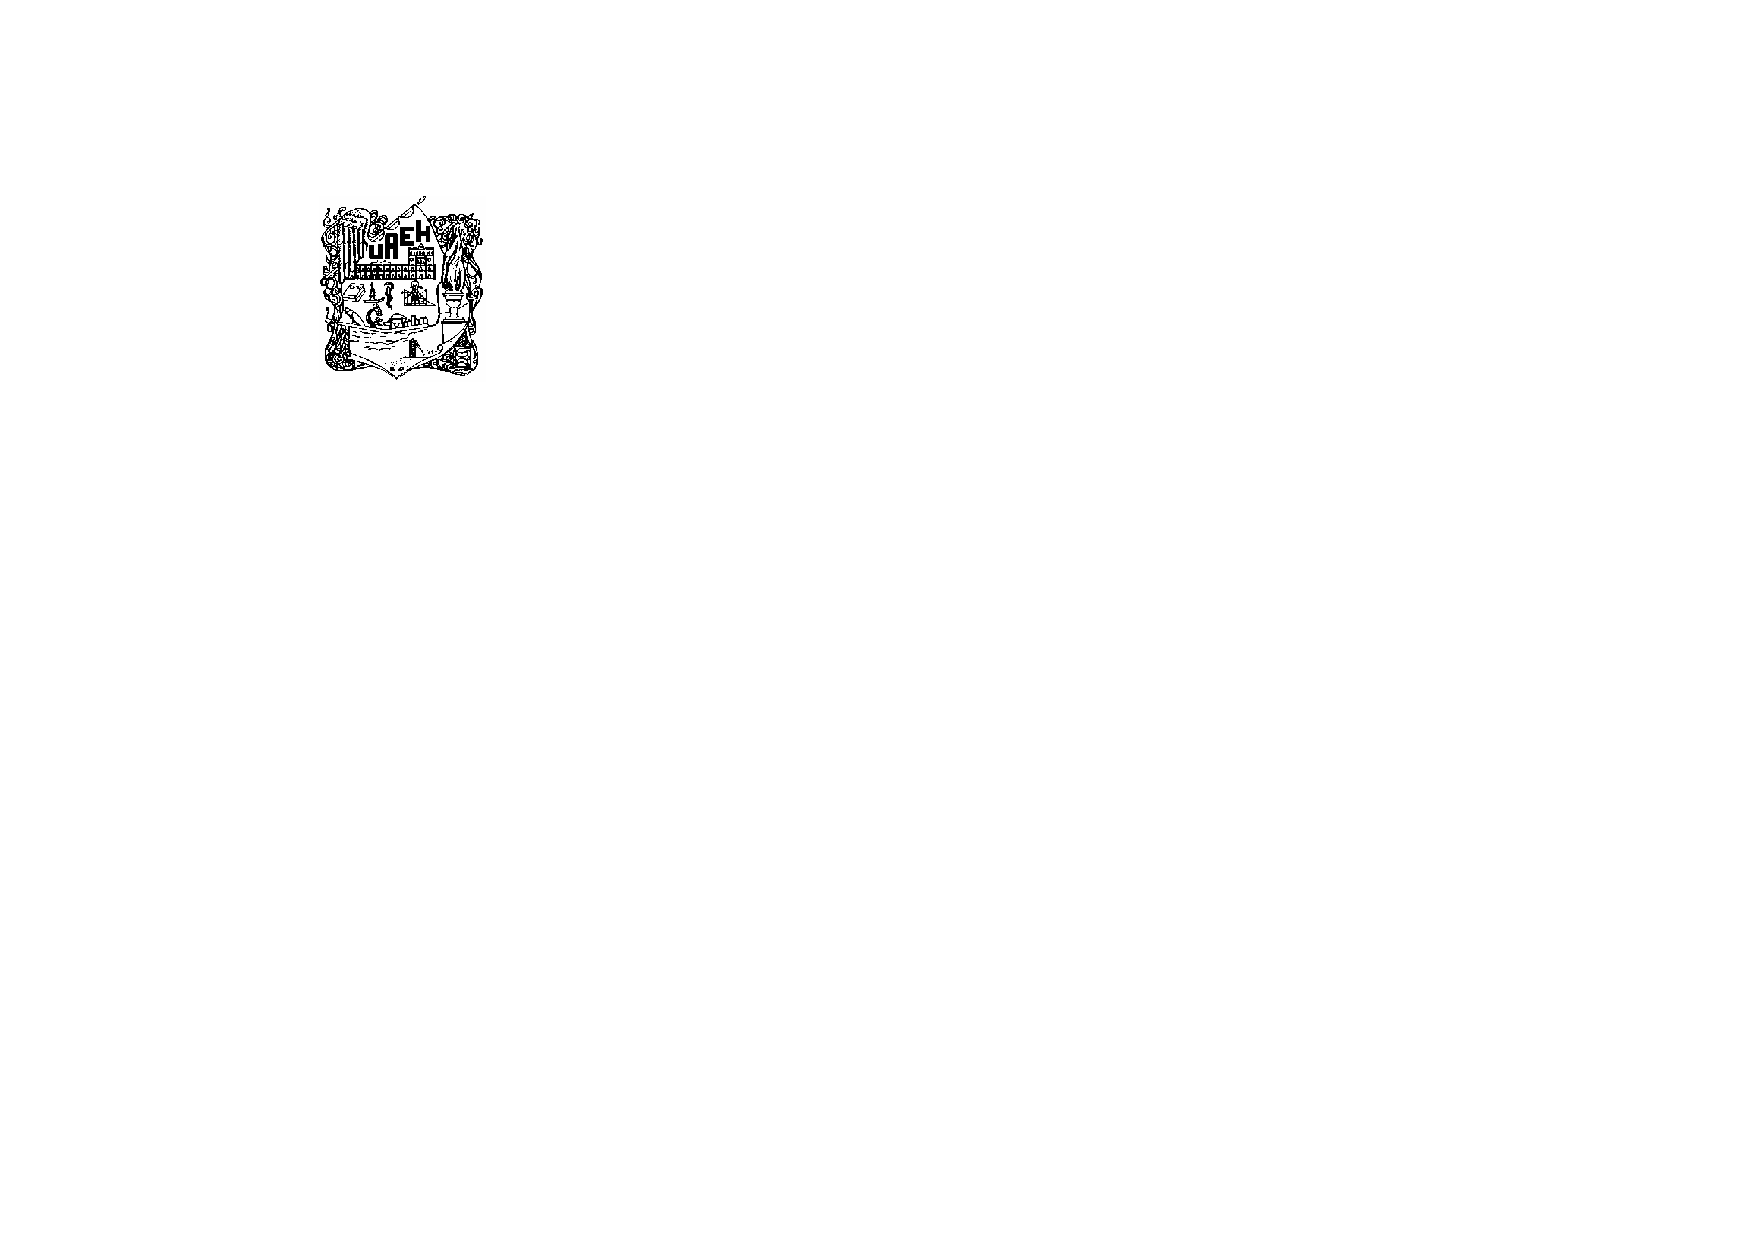
\includegraphics[scale=1.2,bb=55 20 0 0]{escudouaeh.pdf}

    \vspace*{\elespacio}

    \textsc{Universidad Autónoma del Estado de Hidalgo}

    \textsc{Instituto de Ciencias Básicas e Ingeniería}

    \textsc{Área Académica de Matemáticas y Física}

    \vspace*{\elespacio}

    {\Huge\bfseries Un enfoque computacional de representaciones de
      grupos en homologías\par}

    \vspace*{\elespacio}

    {\large Tesis que para obtener el título de}

    \vspace*{\elespacio}

    {\Large\textsc{Licenciado en Matemáticas Aplicadas}}

    \vspace*{\elespacio}

    {\large presenta}

    \vspace*{\elespacio}

    {\Huge Manuel Campero Jurado}

    \vspace*{\elespacio}

    {\large bajo la dirección de}

    \bigskip

    {\Large Dr.~Rafael Villarroel Flores}

    \bigskip

    {Pachuca, Hidalgo. Octubre de 2018.}

    \vspace*{\fill}

  \end{center}
\end{titlepage}

\thispagestyle{empty}
\begin{flushleft}
  {\bfseries\Large Resumen}
\end{flushleft}

En esta tesis se hace blah blah blah blah blah blah blah blah blah
blah blah blah blah blah blah blah blah blah.

\vspace{2cm}

\begin{flushleft}
  {\bfseries\Large Abstract}
\end{flushleft}

In this thesis blah blah blah blah blah blah blah blah blah
blah blah blah blah blah blah blah blah blah.

 \newpage \thispagestyle{empty}

\chapter{Representaciones de grupos}
\label{cha:Representaciones de grupos}

Sea $GL\left(n,\mathbb{C}\right)$ el grupo de todas las matrices no
singulares de grado $n$ sobre el campo de los números complejos
$\mathbb{C}$. Sea $G$ un grupo. Una representación (matricial) de $G$
es, por definición, un homomorfismo de $G$ en
$GL\left(n,\mathbb{C}\right)$: $\mathbb{A}\colon a\mapsto
A\left(a\right)$, tal que:
\begin{enumerate}
\item $A\left(ab\right)\left(a\right)\left(b\right)$,
\item $A\left(1\right)=\mathrm{I}$ (la matriz identidad),
\item $A\left(a^{-1}\right)=A\left(a\right)^{-1}$.
\end{enumerate}
El número $n$ se llama el grado de la representación. Se dice que la
representación es fiel, si $\mathbb{A}$ es biyectiva.

\textbf{Ejemplo 1.1.} El mapeo que a manda cada elemento de $G$ a $1
\in \mathbb{C}$ es una representación de grado 1. Ésta es llamada la
representación unitaria de $G$, y es denotada por $1_{G}$.

\textbf{Ejemplo 1.2.} Dada una representación $a \mapsto A\left(a\right)$, el mapeo
\begin{equation*}
  a \rightarrow P^{-1}A\left(a\right)P
\end{equation*}  
se convierte en una representación de $G$ para cualquier matriz $P$ no singular.

Sean $\mathbb{A} \colon a\mapsto A\left(a\right)$ y $\mathbb{B} \colon
a\mapsto B\left(a\right)$ representaciones de $G$. Si exite una
matriz no singular $P$ tal que
\begin{equation*}
  B\left(a\right)= P^{-1}A\left(a\right)P
\end{equation*}
diremos que $\mathbb{A}$ y $\mathbb{B}$ son
equivalentes. Representaciones equivalentes son denotadas por
$\mathbb{A} \sim \mathbb{B}$. La relación $\sim$ define una clase de
equivalencia de representaciones de $G$.
\textbf{Ejemplo 1.3.} Sea $S_{n}$ el grupo simétrico de grado
$n$. Para un elemento
\begin{equation*}
  \sigma =
  \begin{pmatrix}
    1 & 2 & \cdots  & n\\ 
    s_{1} & s_{2} & \cdots & s_{n}
  \end{pmatrix} 
  \in S_{n}
\end{equation*}  
Sea $A\left(\sigma\right)$ la matriz cuyo $i$-ésimo renglón es
$\left(0,...,0,1,0,...,0\right)$ con 1 en el $s_{i}$-ésimo lugar:
\begin{equation*}
A\left(\sigma\right) = \left(\alpha_{ij}\left(\sigma\right)\right) 
\qquad
\left(i,j=1,2,...,n\right)
\end{equation*}
con
\begin{equation*}
         \alpha_{ij}\left(\sigma\right) = \left\{
	       \begin{array}{ll}
		 1      & \mathrm{si\ } j = s_{i} \\
		 0      & \mathrm{otro\ caso\ } 
	       \end{array}
	     \right.
\end{equation*}
El mapeo $\sigma \mapsto A\left(\sigma\right)$ es una representación
fiel de $S_{n}$.

\textbf{Ejemplo 1.4.} Sea $G$ un grupo finito que
consiste de los elementos $a_{1},a_{2},...,a_{n}$ y sea $S^{G}$ el
grupo simétrico en $G$. El mapeo lleva cada elemento de $a \in G$ a la
permutación
\begin{equation*}
  \begin{pmatrix}
    a_{1} & a_{2} & \cdots  & a_{n}\\ 
    a_{1}a & a_{2}a & \cdots & a_{n}a
  \end{pmatrix} 
  \in S_{n}^{G}
\end{equation*}
es un homomorfismo biyectivo de $G$ a $S^{G}$. A la permutación
anterior, se le asocia la matriz
\begin{equation*}
  A\left(a\right)=\left(\alpha_{ij}\left(a\right)\right)
\end{equation*}
con
\begin{equation*}
         \alpha_{ij}\left(a\right) = \left\{
	       \begin{array}{ll}
		 1      & \mathrm{si\ } a_{i}a = a_{j} \\
		 0      & \mathrm{otro\ caso\ } 
	       \end{array}
	     \right.
\end{equation*}
como en el ejemplo 1.3. Entonces el mapeo
$a \mapsto A\left(\sigma\right)$ convierte una representación fiel de
$G$. Ésta representación es llamada represetación regular derecha de
$G$. Sea $\Delta\left(a\right)$
\begin{equation*}
         \alpha_{ij}\left(a\right) = \left\{
	       \begin{array}{ll}
		 1      & \mathrm{si\ } a = 1 \\
		 0      & \mathrm{otro\ caso\ } 
	       \end{array}
	     \right.
\end{equation*}
entonces
\begin{equation*}
  A\left(a\right) = 
  \begin{pmatrix}
    \delta\left(a_{1}aa_{1}^{-1}\right) & \delta\left(a_{1}aa_{2}^{-1}\right) & \cdots  & \delta\left(a_{1}aa_{n}^{-1}\right)\\
    \delta\left(a_{2}aa_{1}^{-1}\right) & \delta\left(a_{2}aa_{2}^{-1}\right) & \cdots  & \delta\left(a_{2}aa_{n}^{-1}\right)\\ 
    \cdots & \cdots & \cdots & \cdots\\
    \delta\left(a_{n}aa_{1}^{-1}\right) & \delta\left(a_{n}aa_{2}^{-1}\right) & \cdots  & \delta\left(a_{n}aa_{n}^{-1}\right)
  \end{pmatrix} 
\end{equation*}
Si a $\neq$ 1, cada entrada sobre la diagonal es cero.

La representación regular izquierda de $G$ es definida similarmente
usando el homomorfismo
\begin{equation*}
  \begin{pmatrix}
    a_{1} & a_{2} & \cdots  & a_{n}\\ 
    aa_{1} & aa_{2} & \cdots & aa_{n}
  \end{pmatrix}
\end{equation*}
concretamente
\begin{equation*}
  A\left(a\right) = 
  \begin{pmatrix}
    \delta\left(a_{1}^{-1}aa_{1}\right) & \delta\left(a_{1}^{-1}aa_{2}\right) & \cdots  & \delta\left(a_{1}^{-1}aa_{n}\right)\\
    \delta\left(a_{2}^{-1}aa_{1}\right) & \delta\left(a_{2}^{-1}aa_{2}\right) & \cdots  & \delta\left(a_{2}^{-1}aa_{n}\right)\\ 
    \cdots & \cdots & \cdots & \cdots\\
    \delta\left(a_{n}^{-1}aa_{1}\right) & \delta\left(a_{n}^{-1}aa_{2}\right) & \cdots  & \delta\left(a_{n}^{-1}aa_{n}\right)
  \end{pmatrix} 
\end{equation*}
Sea $\phi \colon a \mapsto \phi\left(a\right)$ un homomorfismo de $G$
en $S_{n}$ (es decir, una permutación de de $G$). Expresando la
permutación $\phi\left(a\right)$ por la matriz $A\left(a\right)$ como
en el ejemplo 1.3, se obtiene una matriz representación
$a \mapsto\rightarrow A\left(a\right)$.

Sea $\mathbb{A} \colon a \mapsto A\left(a\right)$ una representación
de grado $n$. Se dice que $\mathbb{A}$ es reducible si existe una
matriz no singular, tal que
\begin{equation*}
  P^{-1}A\left(a\right)P=
  \begin{pmatrix}
    B\left(a\right) & 0 \\
    D\left(a\right) & C\left(a\right)
  \end{pmatrix} 
\end{equation*}  
donde $B\left(a\right)$, $C\left(a\right)$ son matrices cuadradas de
grado $r$, $s$ con $r \geq 1$, $s \geq 1$, $r+s=n$. Se observa que las
representaciones
\begin{equation*}
  a \mapsto A^{'}\left(a\right)=
  \begin{pmatrix}
    B\left(a\right) & 0 \\
    D\left(a\right) & C\left(a\right)
  \end{pmatrix}
\end{equation*}
y
\begin{equation*} 
  a \mapsto A^{''}\left(a\right)=
  \begin{pmatrix}
    C\left(a\right) & D\left(a\right) \\
    0 & C\left(a\right)
  \end{pmatrix}
\end{equation*}
son equivalentes, porque
$Q^{-1}A^{'}\left(a\right)Q=A^{''}\left(a\right)$, con
\begin{equation*}
  Q=
  \begin{pmatrix}
    0 & \mathrm{I_{R}} \\ 
    \mathrm{I_{S}} & 0
  \end{pmatrix} \qquad \mathrm{(I_{r},I_{s}\ son\ las\ matrices\ identidad\ de\ grado\ r,s).\ }
\end{equation*}
Se dice que $\mathbb{A}$ es irreducible si no es reducible. En el
ejemplo 1.3, el mapeo $a \mapsto B\left(a\right)$ y
$a \mapsto C\left(a\right)$ convierten representaciones de grado
$r,s$, respectivamente.

Dada una representación de $G$,
$\mathbb{A} \colon a \mapsto A\left(a\right)$, y
$\mathbb{B} \colon a \mapsto B\left(a\right)$, con grado $n$, $m$,
respectivamente, el mapeo.
\begin{equation*}
  Q=
  \begin{pmatrix}
    A\left(a\right) & 0 \\ 
    0 & B\left(a\right)
  \end{pmatrix}, \qquad \mathrm{para\ todo\ } a \in G
\end{equation*}
convierte en una representación de $G$ de grado $n+m$. Esta
representación es llamada la suma directa de $\mathbb{A}$ y
$\mathbb{B}$, y es denotada por $\mathbb{A}\oplus\mathbb{B}$.

Una representación $\mathbb{A}\colon a \mapsto A\left(a\right)$ de $G$
se dice completamente reducible si $\mathbb{A}$ es equivalente a la
suma directa de algunas representaciones irreducibles, es decir,
existe una matriz no singular $P$, tal que
\begin{equation*}
 P^{-1}A\left(a\right)P=
 \begin{pmatrix}
   \mathrm{F_{1}}\left(a\right) & & & & & 0\\
   & \mathrm{F_{2}}\left(a\right) & & & & \\
   & & . & & & \\
   & & & . & & \\
   & & & & . & \\
   0 & & & & & \mathrm{F_{r}}\left(a\right)
 \end{pmatrix}
\end{equation*}
donde cada $\mathbb{F_{i}}\colon a \mapsto F_{i}\left(a\right)$
$\left(i=1,2,...,r\right)$ es una representación irreducible de $G$.

\subsubsection{Representación por matrices unitarias, y
  representaciones de completamente reducibles de grupos finitos}
Una representación $\mathbb{A}\colon a \mapsto A\left(a\right)$ de $G$
se dice unitaria si $A\left(a\right)$ es una matriz unitaria para todo
$a \in G$, lo cual significa que
$\overline{A\left(a\right)}^{t}A\left(a\right)=\mathrm{I}$. Aquí
$\overline{A\left(a\right)}^{t}$ denota la transpuesta de
$\overline{A}=\left(\alpha_{ij}\right)$, donde
$A=\left(\alpha_{ij}\right)$, y $\overline{\left(\alpha_{ij}\right)}$
es el complejo conjugado de $\left(\alpha_{ij}\right)$. Se pretende
mostrar que cada representación de un grupo finito es equivalente a
una representación unitaria y es completamente reducible.

Una matriz se dice hermitiana si $\overline{A^{t}}=A$, y positiva
definida si $\overline{x}^{t}Ax>0$ para todo vector columna $x$
(distinto de cero).

\textbf{Lema 2.1.} Para cualquier matriz no singular $A$,
$\overline{A\left(a\right)}^{t}A$ es una matriz hermitiana definida
positiva. La suma de matrices hermitianas definidas positivas, también
es hermitiana y definida positiva.

\textbf{Lema 2.2.} Para cualquier matriz hermitiana definida positiva
$A$, existe una matriz triangular superior no singular $C$ tal que
$\overline{C}^{t}AC=\mathrm{I}$.

Lo anterior es cierto, ya que, sea
\begin{equation*}
  A\left(\alpha_{ij}\right) \mathrm{con\ }
  \left(i,j=1,2,...,n\right).
\end{equation*}  
Entonces
\begin{equation*}
  \alpha_{ji}=\overline{\alpha_{ij}} \quad \mathrm{con\ }
  \left(i,j=1,2,...,n\right),
\end{equation*}
y
\begin{equation*}
\left(\alpha_{ii}\right)>0 \quad \mathrm{para\ }
\left(i=1,2,...,n\right).
\end{equation*}
Sea
\begin{equation*}
  A=
  \begin{pmatrix}
    \alpha & a \\ 
    \overline{a}^{t} & \mathrm{B}
  \end{pmatrix}, \quad \left(\alpha=\alpha_{11}>0,
    a=\left(\alpha_{12},\alpha_{13},...,\alpha_{1n}\right),
    \mathrm{B}=\left(\alpha_{ij}\right) \quad \left(i,j=2,...,n\right) \right)
\end{equation*}
sea
\begin{equation*} 
  C_{1}=
  \begin{pmatrix}
    \frac{1}{\sqrt{\alpha}} & -\frac{1}{\alpha} \\ 
    0 & \mathrm{I}
  \end{pmatrix}
\end{equation*}
entonces, 
\begin{equation*}
  \overline{C_{1}}^{t}AC_{1} =
  \begin{pmatrix}
    1 & 0 \\ 
    0 & -\frac{1}{\alpha}\overline{a}^{t}a+\mathrm{B}
  \end{pmatrix}
\end{equation*}  
y $-\frac{1}{\alpha}\overline{a}^{t}a+\mathrm{B}$ es una matriz
hermitiana definida positiva. Y la prueba se sigue usando inducción el
grado de $A$ veces.

\textbf{Teorema 2.3.} Sea $G$ un grupo finito. Para una representación
$\mathbb{B}: a\rightarrow F\left(a\right)$ de $G$, entonces exite una
matriz triangular superior no singular $C$, tal que
$C_{-1}F\left(a\right)C$ es una matriz unitaria para todo $a \in G$.

Sea
\begin{equation*}
A=\sum_{b \in G} \overline{F\left(b\right)}^{t}F\left(b\right)
\end{equation*}
Entonces $A$ es una matriz hermitiana definida positiva por el Lemma
2.1. Entonces existe una matriz triangular no singular $C$, tal que

\begin{equation*}
  \overline{C}^{t}AC= \mathrm{I}
\end{equation*}
\begin{equation*}
  A=\left(\overline{C}^{t}\right)C^{-1}
\end{equation*}
Entonces
\begin{equation*}
\overline{F\left(a\right)}^{t}AF\left(a\right)=\sum_{b \in G} \overline{F\left(ba\right)}^{t}F\left(ba\right)=A
\end{equation*},
y se obtiene
\begin{equation*}
\overline{F\left(a\right)}^{t}(\overline{C}^{t})^{-1}C^{-1}F\left(a\right)=(\overline{C}^{t})^{-1}C^{-1}
\end{equation*},
es decir\\~\\
\begin{equation*}
\overline{(C_{-1}F(a)C)}^{t}(C_{-1}F(a)^{t}C)=\mathrm{I}
\end{equation*}
y $C_{-1}F(a)^{t}C$ es una matriz unitaria.

\textbf{Teorema 2.4.} Una representación de un grupo finito es
completamente reducible.

Sea $\mathbb{A}:$ $a\rightarrow A\left(a\right)$ una representación de
un grupo finito de $G$ y sea $A(a)$ descompuesta como
\begin{equation*}
  A(a)=
  \begin{pmatrix}
    A_{1}(a) & * \\ 
    0 & A_{2}(a)
  \end{pmatrix}
\end{equation*}  
Por el teorema anterior, existe una matriz triangular no superior $C$
tal que $C^{-1}A(a)C$ es una matriz unitaria. Sea
$U(a)=C^{-1}A(a)C$. Como $C$ es una matriz triangular superior, $U(a)$
se descompone como
\begin{equation*}
  U(a)=
  \begin{pmatrix}
    U_{1}(a) & V(a) \\ 
    0 & U_{2}(a)
  \end{pmatrix}
\end{equation*}  
Como $\overline{U(a)}^{t}=U(a)^{-1}=U(a^{-1})$, se obtiene
\begin{equation*}
  \begin{pmatrix}
    \overline{U_{1}(a)} & 0 \\ 
    \overline{V(a)}^{t} & \overline{U_{2}(a)}^{t}
  \end{pmatrix}
  =
  \begin{pmatrix}
    U_{1}(a^{-1}) & V(a^{-1}) \\ 
    0 & U_{2}(a^{-1})
  \end{pmatrix}
\end{equation*}  
\textbf{Lema 3.1.} (Lema de Schur) Sea
$\mathbb{A} \colon a \mapsto A\left(a\right)$ y
$\mathbb{B} \colon a \mapsto B\left(a\right)$ representaciones
irreducibles de un grupo $G$ con grados $m$ y $n$ respectivamente. Sea
$P$ una matriz de $m$x$n$ con la propierdad de que $A(a)P=PB(a)$, para
todo $a \in G$.
entonces
\begin{itemize}
\item $P=0$
\item $m=n$ y $P$ es no singular.
\end{itemize}
Asumimos $P \neq 0$. Y se quiere mostrar la segunda
condición. Supongamos que $m \neq n$, o $m=n$ y $P$ es
singular. Entonces existe $Q \in GL(m,\mathbb{C})$ y
$\mathrm{R} \in GL(n,\mathbb{C})$, tal que
\begin{equation*}
  QPR=
  \begin{pmatrix}
    \mathrm{I_{r}} & 0 \\ 
    0 & 0
  \end{pmatrix} \quad \mathrm{(I_{r},\ es\ la\ matriz\ identidad\ de\ grado\ r).\ }
\end{equation*}  
con $r<$max$\left\{ m,n \right\}$. Como $QA(a)Q^{-1}(QPR) = QPR(R^{-1}B(a)R)$, y se obtiene
\begin{equation*}
  \begin{pmatrix}
    A_{11} & 0 \\ 
    A_{21} & 0
  \end{pmatrix}
  =
  \begin{pmatrix}
    B_{11} & B_{12} \\ 
    0 & 0
  \end{pmatrix},
\end{equation*}
donde
\begin{equation*}
  QA(a)A^{-1}=
  \begin{pmatrix}
    A_{11} & A_{12} \\ 
    A_{21} & A_{22}
  \end{pmatrix} \quad \mathrm{(A_{11},\ es\ una\ matriz\ cuadrada\ de\ grado\ r).\ }
\end{equation*}  
y
\begin{equation*}
  R^{-1}B(a)R=
  \begin{pmatrix}
    B_{11} & B_{12} \\ 
    B_{21} & B_{22}
  \end{pmatrix} \mathrm{(B_{11},\ es\ una\ matriz\ cuadrada\ de\ grado\ r).\ }
\end{equation*}  
Por lo tanto $A_{21}=0$ si $r<m$ y $B_{12}$ si $r<n$. De cualquier
manera $\mathbb{A}$ o $\mathbb{B}$ es reducible, lo cual es una
contradicción.

\textbf{Teorema 3.2.} Sea
$\mathbb{A} \colon a \mapsto A\left(a\right)$ una representación
irreducible de un grupo $G$. Sea $P$ una matriz con la propiedad
$A(a)P=PA(a)$ para todo $a \in G$. Entonces $P=\lambda \mathrm{I}$,
para algún $\lambda \in \mathbb{C}$.

Sea $\lambda$ un eigenvalor de $P$. Entonces
det$(\lambda \mathbb{I} - P)=0$, y además

\begin{equation*}
  A(a)(\lambda \mathbb{I} - P)=(\lambda \mathbb{I} - P)A(a) \qquad \mathrm{(para\ todo\ a \in G.)}
\end{equation*}
Entonces por el Lema de Schur,
\begin{equation*}
  \lambda \mathrm{I}-P=0
\end{equation*}
\textbf{Teorema 3.2.} Sea $G$ un grupo abeliano. Entonces cada
representación irreducible de $G$ es de grado 1.

Sea $\mathbb{A}\colon a \mapsto A\left(a\right)$ una representación
irreducible de $G$. Como $A(a)$ conmuta con $A(b)$, el teorema pasado
nos dice que $A(a)=\lambda(a) \mathrm{I}$ para algún
$\lambda(a) \in \mathbb{C}$. Entonces $\mathbb{A}$ es irreducible, y
el grado de $\mathbb{A}$ debe ser 1.

\textbf{(Relación ortogonal de carácteres).} Desde aquí en adelante,
se asumirá que estamos trabajando con grupos finitos.

\textbf{Carácteres} Para una matriz cuadrada $A=\alpha_{ij}$ de grado
$n$, $\mathrm{tr\ A}$ denota la traza de $A$, es decir
\begin{equation*}
  \mathrm{tr\ A}=\alpha_{11}+\alpha_{22}+ \cdots \alpha_{nn}
\end{equation*}
Cálculos directos muestran que
\textbf{Lema 4.1. }
\begin{itemize}
\item $\mathrm{tr\ AB}=\mathrm{tr\ BA}$
\item $\mathrm{tr\ P^{-1}AP}=\mathrm{tr\ A}$ para alguna matriz no singular $P$.
\end{itemize}

Para una representación $\mathbb{A} \colon a \mapsto A\left(a\right)$
de un grupo $G$, sea $\mathrm{tr\ A(a)}=\chi(a)$. Entonces $\chi(a)$
es una función que toma valores en $\mathbb{C}$ y es llamada el
carácter de $\mathbb{A}$. Obviamente, $\chi(1)$ es igual al grado de
$\mathbb{A}$. Carácteres de representaciones irreducibles son llamados
carácteres irreducibles. Y por el lema 4.1(2), se tiene lo siguiente:

\textbf{LEMA 4.2. } Representaciones equivalentes de un grupo tienen
el mismo carácter.

Como $A(x^{-1}ax)=A(x)^{-1}A(a)A(x)$, se sigue que
\begin{equation*}
  \chi(x^{-1}ax)=\chi(a)
\end{equation*}  
Así $\chi$ toma el mismo valor en una clase de conjugación de $G$. Tal
función es llamada función de clase.

\textbf{La primera relación ortogonal de carácteres.} Sea $G$ un grupo
de orden $g$. Sean
$\mathbb{A} \colon a \mapsto A\left(a\right) = (\alpha_{ij}(a))$, y
$\mathbb{B} \colon a \mapsto B\left(a\right) = (\alpha_{ij}(a))$
representaciones irreducibles de $G$ con grado $m,n$,
respectivamente. Para una matriz arbitraria $U=(\gamma_{ij})$, de
$m$x$n$, se tiene

\begin{equation*}
 V=\sum_{x \in G} A(x)UB(x^{-1}).
\end{equation*}
Entonces
\begin{equation*}
  \begin{aligned}
    A(a)V &=\sum_{x \in G} A(ax)UB(x^{-1})\\
    &=\sum_{y \in G} A(y)UB(y^{-1}a) \qquad (y=ax)\\
    &=\sum_{y \in G} A(y)UB(y^{-1})B(a).
  \end{aligned}
\end{equation*}
Como $y$ varia sobre $G$ conforme $x$ lo hace, 	se tiene
\begin{equation*}
  A(a)V=VB(a).
\end{equation*}  
Asuminos que $A$ y $B$ no son equivalentes. Entonces $V=0$ por el Lema
de Schur. La $(ij)$ entrada de $V$ es

\begin{equation*}
 \sum_{x \in G} \quad \sum_{u,v} \alpha_{iu}(x) \gamma_{uv} \beta_{vj}(x^{-1}) = 0.
\end{equation*}
En particular, para algún par de $u$,$v$ sea $\gamma_{uv}=1$ y para
cualquier otro caso $\gamma_{\rho \sigma}=0$. Lo cual conduce a

\begin{equation*}
  \sum_{x \in G} \alpha_{iu}(x) \beta_{vj}(x^{-1}) = 0.
\end{equation*}
Ahora, asumimos que $\mathbb{A}=\mathbb{B}$. Entonces para algún
$\lambda \in \mathbb{C}$, $V=\lambda\mathrm{I}$, y por el Teorema
3.2. La $(i,j)$ entrada de $V$ es

\begin{equation*}
\qquad \sum_{x \in G} \quad \sum_{u,v} \alpha_{iu}(x) \gamma_{uv} \beta_{vj}(x^{-1}) = \delta_{ij}\lambda,
\end{equation*}
donde $\delta_{ii}=1$, $\delta_{ij}=0$ ($i \neq j$). Tomando la traza de
\begin{equation*}
\qquad \sum_{x \in G} A(x)UA(x^{-1}) = \lambda \mathrm{I}
\end{equation*}
y se obtiene
\begin{equation*}
  g(\gamma_{11}+\gamma_{22}+ \cdots +\gamma_{nn})
\end{equation*}  
donde $n$ es el grado de $\mathbb{A}$,y $g$ es la cardinalidad de $G$, de lo cual se sigue

$\lambda=\frac{g}{n}(\gamma_{11}+\gamma_{22}+ \cdots + \gamma_{nn})$.

Ahora, para algún par de $u$,$v$ sea $\gamma_{uv}=1$ y para cualquier otro caso $\gamma_{\rho \sigma}=0$. Entonces
\begin{equation*}
  \sum_{x \in G} \alpha_{iu}(x) \beta_{vj}(x^{-1}) = \delta_{ij} \delta_{uv}\frac{g}{n}.
\end{equation*}
Lo cual nos conduce al siguiente teorema

\textbf{Teorema 4.3. } Sea $G$ un grupo de orden $g$.
\begin{itemize}
\item Sea $\mathbb{A}: a \rightarrow A(a)=(\alpha_{ij}(a))$ una
  representación irreducible de $G$ con grado $n$. Entonces
\end{itemize}
\begin{equation*}
\sum_{x \in G} \alpha_{iu}(x) \alpha_{vj}(x^{-1}) = \delta_{ij} \delta_{uv}\frac{g}{n}.
\end{equation*}
\begin{itemize}
\item Sea $\mathbb{B}:b \rightarrow B(a)=(\beta_{ij}(a))$ una
  representación irreducible, la cual no es esquivalente a
  $\mathbb{A}$, entonces
\end{itemize}
\begin{equation*}
\sum_{x \in G} \alpha_{iu}(x) \beta_{vj}(x^{-1}) = 0.
\end{equation*}
Sean $\chi$, $\chi^{'}$ los carácteres de $\mathbb{A}$,
$\mathbb{B}$. Por el teorema anterior, poniendo a $u=i$, $v=j$ y
tomando la suma sobre $i$,$j$, se obtiene lo siguiente:

\textbf{Teorema 4.4. } (La primer relación de ortogonalidad de
carácteres) Sea $G$ un grupo de orden $g$.
\begin{itemize}
\item Sea $\chi$ un caráter irreducible de $G$, entonces 
\end{itemize}
\begin{equation*}
\sum_{x \in G} \chi(x) \chi(x^{-1}) = g.
\end{equation*}
\begin{itemize}
\item Sea $\chi$, $\chi^{'}$ carácteres de representaciones
  irreducibles no equivalentes de $G$, entonces
\end{itemize}
\begin{equation*}
\sum_{x \in G} \chi(x) \chi^{'}(x^{-1}) = 0.
\end{equation*}
Se observa que $\chi(a^{-1})=\overline{\chi(a)}$ para todo $a \in G$,
porque el Teorema 2.3 dice que $\mathbb{A}$ es equivalente a una
representación unitaria $\mathbb{U}\colon a \mapsto U(a)$, y se por lo
tanto
\begin{equation*}
\chi(a^{-1})=trU(a^{-1})=trU(a)^{-1}=tr \overline{U(a)}^{t} = \overline{\chi(a)}  
\end{equation*} 
Sean $\mathbb{F}_{1}$, $\mathbb{F}_{2}$,... representantes de las
clases de equivalencia de las representaciones irreducibles de un
grupo $G$ y sea $\chi_{1}$, $\chi_{2}$,... los carácteres de
$\mathbb{F}_{1}$, $\mathbb{F}_{2}$,... .  Sea $C_{1}$,
$C_{2}$,...,$C_{k}$ las clases de conjuación de $G$ con
$|C_{\alpha}|=h_{\alpha}$ ($\alpha=1, 2, 3,...,k$) y sea $a_{1}$,
$a_{2}$,...,$a_{k}$ los representantes de las clases de
conjugación. Como los carácteres son funciones de clases, el Teorema
4.4 se reescribe como sigue

\textbf{Theorema 4.4'. }
\begin{equation*}
\sum_{\alpha=1}^{k} h_{\alpha} \chi_{i}(a_{\alpha}) \overline{\chi_{j}(a_{\alpha})} = \delta_{ij}g.
\end{equation*}
Para funciones $\varphi$, $\psi$ que toman valores en $\mathbb{C}$ en
un grupo $G$ de orden $g$, se define el producto interno
$(\varphi,\psi)_{G}$ de la siguiente manera
\begin{equation*}
(\varphi,\psi)_{G} = \frac{1}{g} \sum_{x \in G} \varphi(x) \psi(x^{-1})
\end{equation*}
Cuando sea claro que se está hablando del grupo $G$, se escribirá
$(\varphi,\psi)$ en lugar de $(\varphi,\psi)_{G}$. Claramente el
producto interno cumple las siguientes propiedades
\begin{equation*}
(\varphi,\psi)=(\psi,\varphi),\\
(\varphi_{1}+\varphi_{2},\psi)=(\varphi_{1},\psi)+(\varphi_{2},\psi),\\
(\varphi,\psi_{1}+\psi_{2})=(\varphi,\psi_{1})+(\varphi,\psi_{2}),\\
(\lambda \varphi,\psi)=(\psi,\lambda \varphi)=\lambda (\varphi,\psi).
\end{equation*}
Con esta notación la primera relación de ortogonalidad de carácteres
es expresada como sigue:

\textbf{Teorema 4.4''. } Sean $\chi_{1}$, $\chi_{2}$,... los
carácteres de carácteres de representaciones no equivalentes de un
grupo $G$. Entonces
\begin{equation*}
(\chi_{i},\chi_{j})=\delta_{ij}
\end{equation*} 
Multiplicidad de representaciones irreducibles. Sea $\mathbb{A}$ una
representación de un grupo $G$. Como $\mathbb{A}$ es completamente
reducible, entonces por el Teorema 2.3, $\mathbb{A}$ es equivalente a
\begin{equation*}
\begin{aligned}
\begin{pmatrix}
\mathbb{F}_{1} & & & & & & 0\\ 
 & \ddots & & & & & \\
 & & \mathbb{F}_{1} & & & & \\
 & & & \mathbb{F}_{2} & & & \\
 & & & & \ddots & & \\
 & & & & & \mathbb{F}_{2} & \\
0 & & & & & & \ddots
\end{pmatrix},
\end{aligned}
\end{equation*}
donde $\mathbb{F}_{1}$, $\mathbb{F}_{2}$,... son representaciones no
equivalentes. El número $m_{i}$ es llamado la multiplicidad de
$\mathbb{F}_{i}$ en $\mathbb{A}$ ($m_{i}=0$ si $\mathbb{F}_{i}$ no
aparece) y se escribe
\begin{equation*}
\mathbb{A} \sim m_{1} \mathbb{F}_{1}+m_{2} \mathbb{F}_{2}+ \cdots
\end{equation*}
Sea $\chi$ el caráter de $\mathbb{A}$ y $\chi_{i}$ el carácter de $\mathbb{F}_{i}$ ($i = 1, 2, ...$). Entonces
\begin{equation*}
\chi =m_{1} \chi_{1}+ m_{2} \chi_{2}+ \cdots
\end{equation*}
Si $m_{i} \neq 0$, $\mathbb{F}_{i}$ y $\chi_{i}$ son llamados
componentes irreducibles de $\mathbb{A}$ y $\chi$ respectivamente.

\textbf{Teorema 4.5. } Sea $G$ un grupo y sea $\chi$ el caráter de una
representación de $G$. Sea $m_{i}$ la multiplicidad de un carácter
irreducible $\chi_{i}$ en $\chi$. Entonces
\begin{equation*}
m_{i} = (\chi,\chi_{i}) = \frac{1}{g} \sum_{x \in G} \chi(x) \overline{\chi_{i}(x)}
\end{equation*}
Sea $$\chi=\sum_{j} m_{j} \chi_{j}$$ la suma de carácteres
irreducibles con $m_{j}$ la multiplicidad de $\chi_{j}$. Entonces
\begin{equation*}
(\chi,\chi_{i}) = \sum_{j} m_{j} (\chi_{j},\chi_{i})
\end{equation*}

\backmatter

\bibliographystyle{plain}
\bibliography{labiblio}

\printindex


\end{document}
